%%%%%%%%%%%%%%%%%%%%%%
\section{Method}
%
%%%%%%%%%%%%%%%%%%%%%%

Compared to the existing works, we noticed that while looking at repositories of satellite imagery that cloudless imagery is quite rare and not feasible to parse on a global scale, since a lot of areas are missing. This is one of the reasons that we chose to use the single channel image data from Sentinel 1A, which is not affected by weather. Another disadvantage we had with our data set is that the resolution is quite low, and glare make it at times impossible \\

To lack of resolution and clarity made it hard to discern the shape of a windmill and thus to train a neural net to identify the distinct shape of a windmill. We therefor decided to focus on detecting parks instead of individual windmills.

\subsection{Satellite Imagery Conversion}

In order to be sure we could re-use our code we decided to re-project the satellite file to the World Geodetic System 1984 - WGS84 (EPSG:4326) 

\begin{lstlisting}[language=Python,breaklines=true]
gdalwarp -t_srs EPSG:4326 in_f out_f
\end{lstlisting}

This also proved necessary due to the warped nature of the raw satellite imagery. By re-projecting the imagery to a fixed coordinate space we could easily switch between coordinates and pixel positions by using existing libraries. 

\subsection{Dataset Creation}

As mentioned before the dataset from which we started is the Sentinel 1A satellite imagery. Since we did not have any labeled data we had to create one ourselves.

\subsubsection{Manual Labeling}

To create a manual labeled set we gathered a collection of coordinates including boats, land and windmills. This can be easily done in mapping software (e.g. QGIS). Once we had our set of coordinates we could start training it model. The model would extract tiles on the coordinates and use those images as training data. We quickly noticed that the amount of samples was not enough (around 150). So we looked at a way of increasing the number of samples.

\subsubsection{Assisted Labeling}

The issue with our first data set was that its size causing a lot of wrong identifications. This bad model actually gave us a great way of creating more samples. We expanded the number of samples we had by saving all right and wrongly identified windmills. To include data like oceans and beaches we would randomly sample at different locations. To ensure a high quality of our samples we also review each one to make sure they clearly identified the object they were representing and that they were centered. \\

To reduce loading times we would save each sample as an image instead of coordinate, making it possible to load our data set without the need of the original satellite image. \\

\begin{figure}[ht]
\begin{center}
\centerline{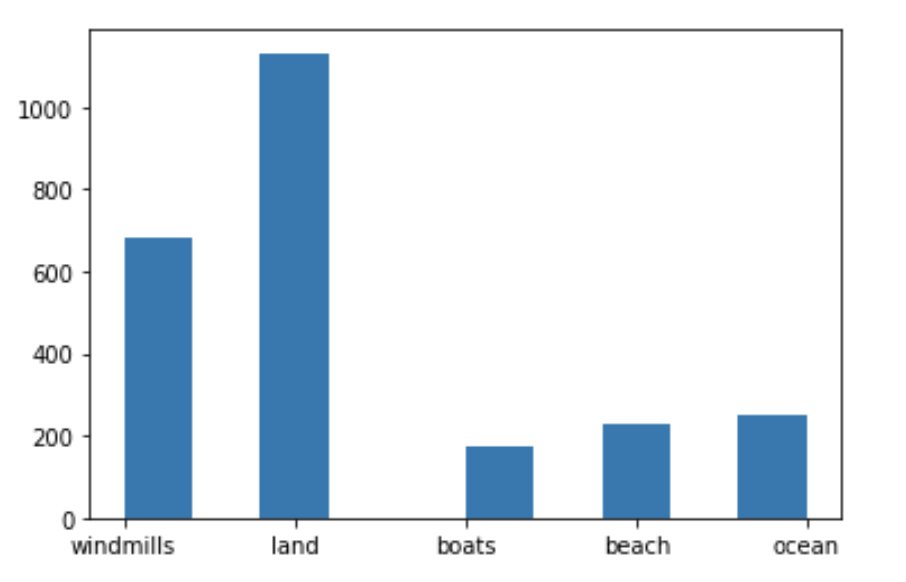
\includegraphics[width=\columnwidth]{images/dataset-stats.png}}
\caption{Statistics of final data set showing the number of examples of each category of classification class.}
\label{dataset-statistics}
\end{center}
\end{figure}

One might notice a large difference between the number of samples (fig. \ref{dataset-statistics}) per category. This was largely due to us wanting to initially train a model that could differentiate between land and non-land images. Due to difficulties of training such model samples of land would not be used in the final result. We tried to have an even amount of samples representing windmill and non-windmill tiles.

\subsection{Noise reduction using OpenCV}

\begin{figure}[ht]
\begin{center}
\centerline{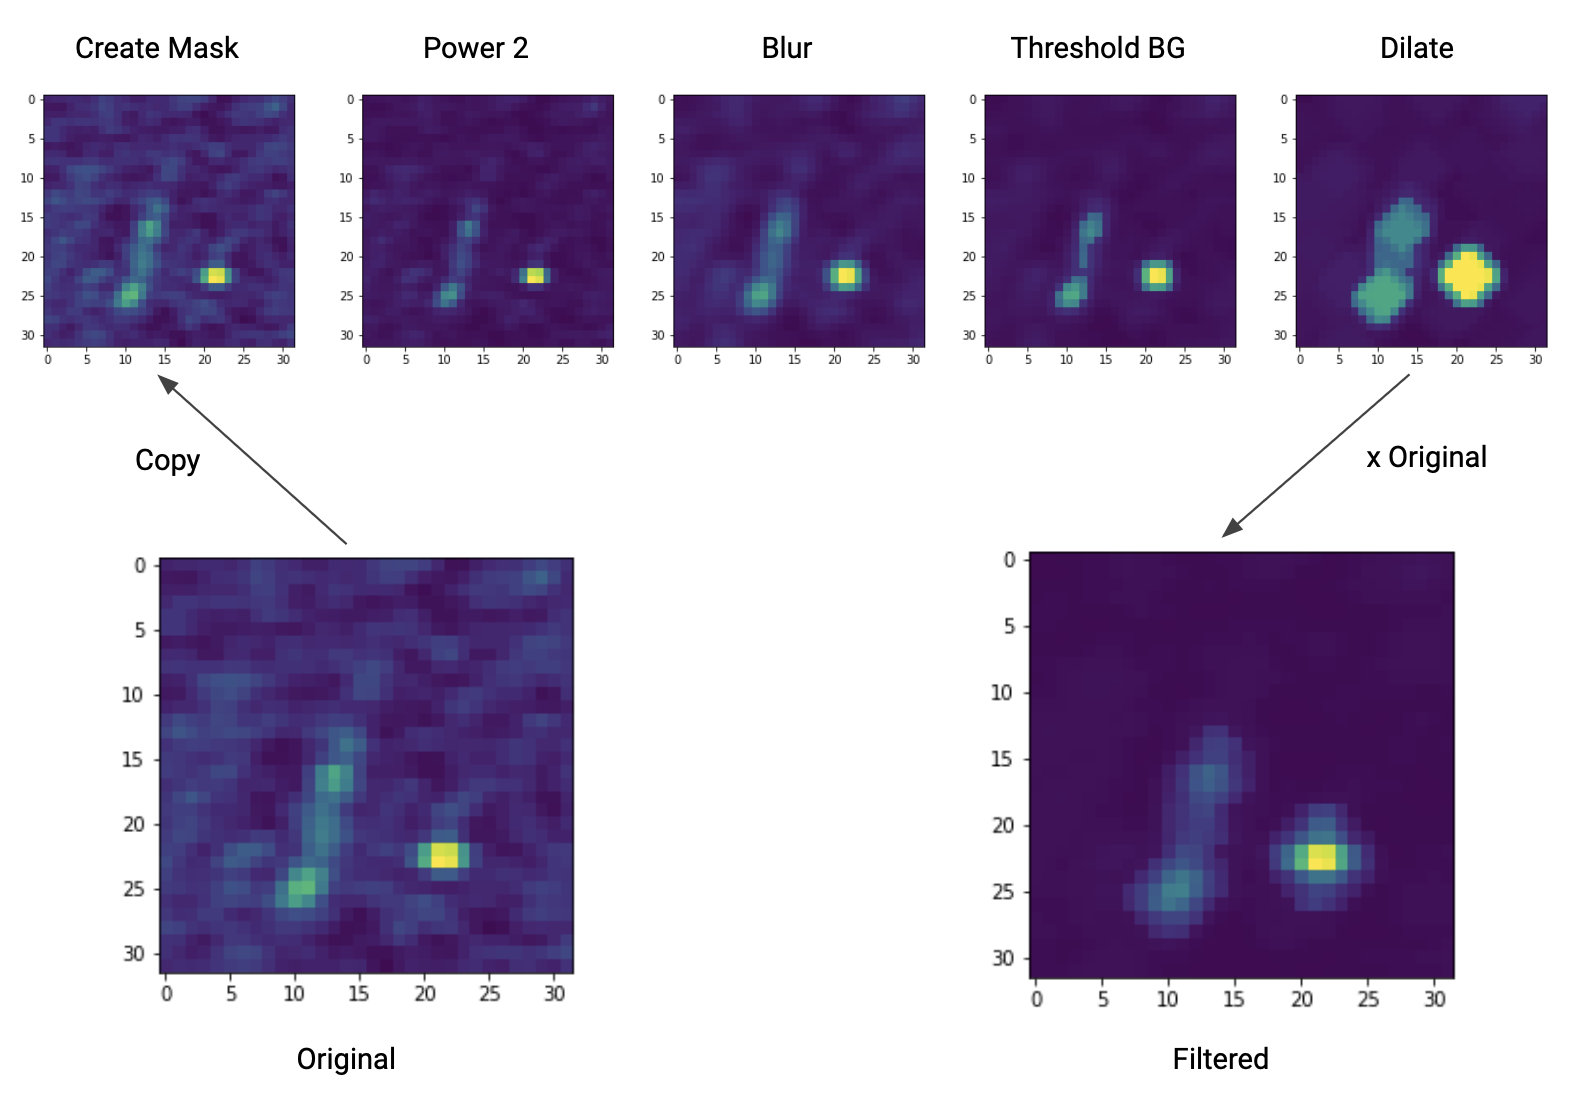
\includegraphics[width=\columnwidth]{images/noise-reduction.png}}
\caption{Step by step process of removing noise from a tile containing a single windmill example.}
\label{noise-reduction}
\end{center}
\end{figure}

We noticed that depending on where the image the intensity of the image might be significantly different. To address this we would pre-process all images before feeding them to our neural network. By masking images in our data set we noticed a more consistent result in training. Without it was noticeable that when adding new samples our model would randomly train better or worse. By masking we would get more consistent results, however this was not empirically tested.\\

The masking itself was done using the OpenCV library. It consists of 4 steps (fig. \ref{noise-reduction}):

\begin{itemize}
    \item Take the power, increasing highlights and decreasing the background.
    \item Apply a $3x3$ blur kernel, removing small artifacts
    \item Remove the background by nullifying values below the avg value
    \item Dilate remaining features to include edges
\end{itemize}

We would then multiply the mask with our original image creating a nice mask around the windmill or boat tile. When using land or ocean imagery we noticed that this would amplify the amount of noise (fig. \ref{noise-reduction-results}).

\subsection{Labeling ocean objects using a CNN}

\subsubsection{Optimal Network}

Before we started designing the topology of our neural network we first looked online to see if there are any example typologies that would be usable for our application. One article we found showed a working neural net to identify boats \cite{moraite_2019}. Whilst the article used color satellite imagery and we are used single channel, the network itself was a good basis to build on. The network however did not produce that good of results. We suspect that this is due to the very different shapes that windmills and boat can have depending on where and when the image was taken. \\

By tweaking the hyper-parameters however and increasing the number of filters to store more information in our network we were able to train a satisfactory model. We tweaked our parameters in a way that our model would be able to detect most windmills and boats but exclude any beaches or other artifacts present in the ocean. Each convolutions layer uses relu as its activation function. Our model had less artifacts when using a 2 class output, this is why we reduce our network to two final nodes, using sigmoid in the final step. The topology is as followed:

\begin{itemize}
    \item Conv2D(32, 5x5)
    \item Pool2D(2x2)
    \item Conv2D(64, 5x5)
    \item Pool2D(2x2)
    \item Flatten()
    \item Dropout(0.5)
    \item Dense(2)
\end{itemize}

All steps contribute to a the stable training of our model. The introduction most notably fixed our issue of over-fitting that was initially noticeable with our small data set. For our result we settled on using the weights at 75 epochs, the moment that our loss would stop decreasing (fig. \ref{cnn-final}) for our test set. 

\begin{figure}[ht]
\begin{center}
\centerline{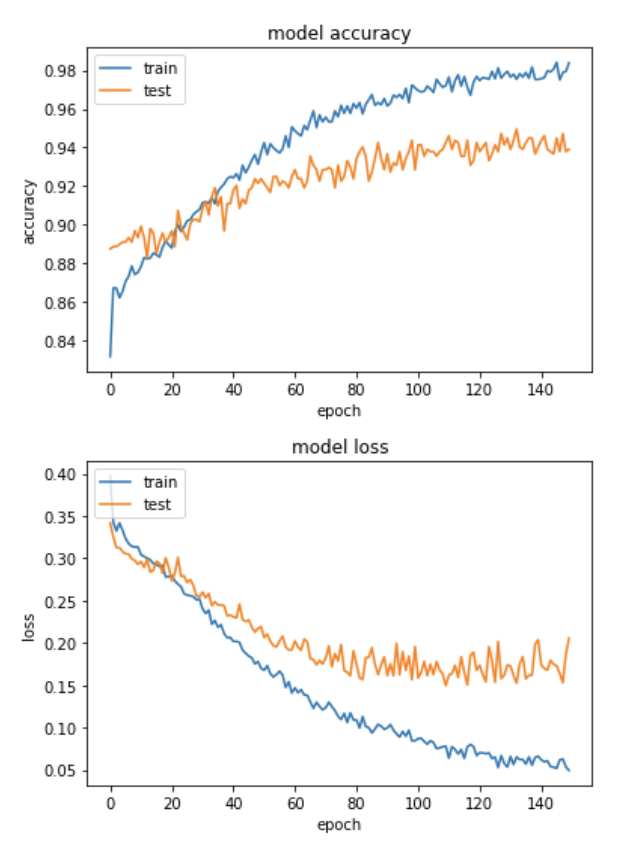
\includegraphics[width=\columnwidth]{images/cnn-training-final.png}}
\caption{Training statistics of our final model.}
\label{cnn-final}
\end{center}
\end{figure}

Looking at our confusion matrix (fig. \ref{bin-confusion}) we see that the model occasionally makes mistakes but these will be filtered away in the next step of our pipeline. One might notice that the amount of water-class examples is less than the object-class. This difference is due to the fact that examples of ocean tiles are mostly noise, adding more noisy ocean tiles did not improve our results, so we did not extract any more samples.

\begin{figure}[ht]
\begin{center}
\centerline{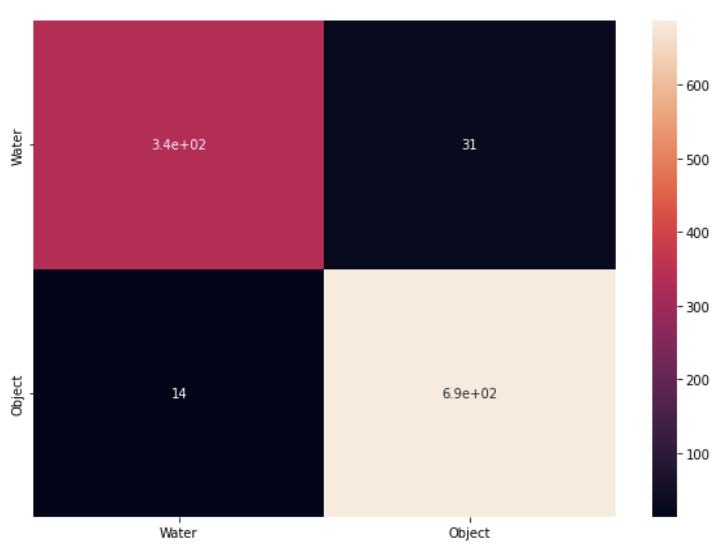
\includegraphics[width=\columnwidth]{images/bin-confusion.png}}
\caption{Confusion matrix of our final CNN.}
\label{bin-confusion}
\end{center}
\end{figure}

\subsubsection{Alternative: Multi-class}

As we mentioned we chose to train our model on two classes instead of the original 5 we designed our dataset for. For completeness sake we included the results of our initial network using 5 classes. The training results look similar, however we achieve a significantly lower accuracy and much higher loss in comparison to using two classes (fig. \ref{cnn-multi}). Also note that land examples are excluded since land noise looks very similar to ocean noise and would decrease our accuracy even more.

\begin{figure}[ht]
\begin{center}
\centerline{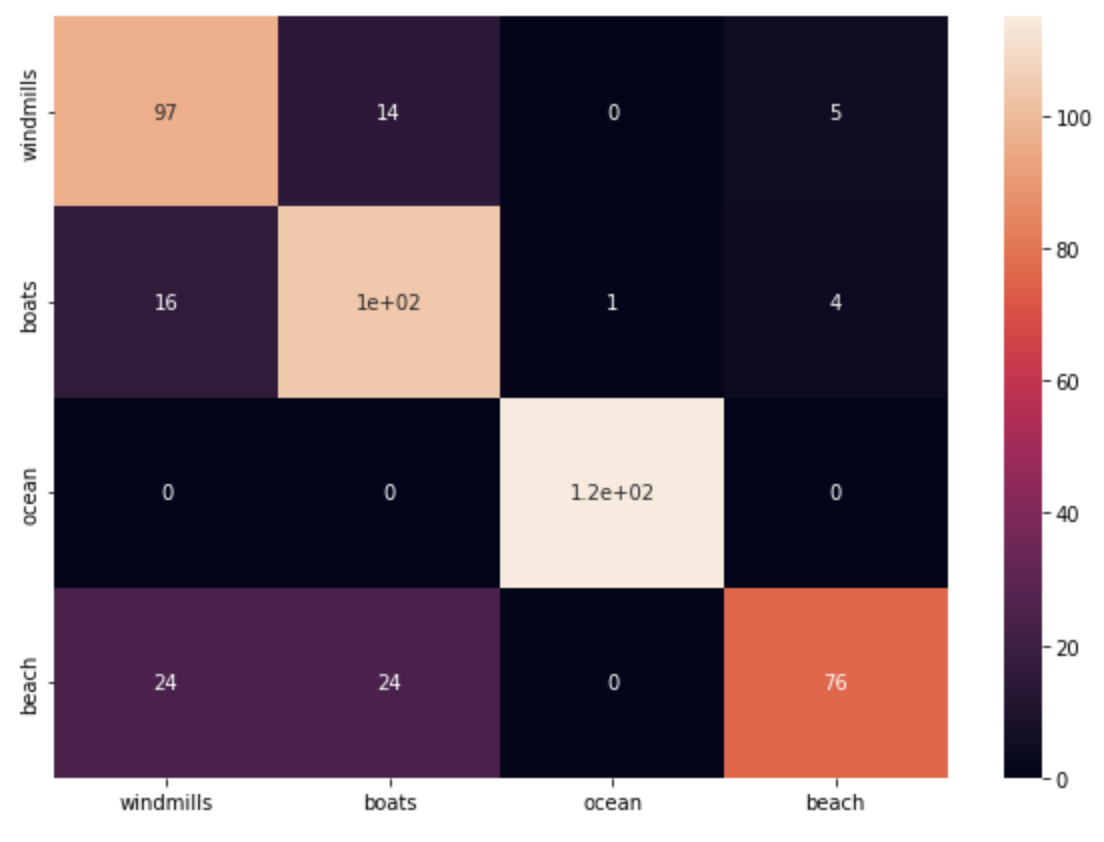
\includegraphics[width=\columnwidth]{images/mul-confusion.png}}
\caption{Confusion matrix using the same topology as our best performing network but modified for multi-classification.}
\label{mul-confusion}
\end{center}
\end{figure}

Looking at the confusion matrix we can see that it is hard to differentiate beaches from boats and windmills. This is an issue that is hard to resolve since beaches have random patterns that sometimes produce artifacts approximating what one would identify as a boat or windmill.\\

What one can also notice is that boats and windmills can be differentiated quite well. However we noticed in later tests that the shape of windmills varies greatly between satellite snapshots and that in reality windmills will have a boat-like shape in most cases.

\begin{figure}[ht]
\begin{center}
\centerline{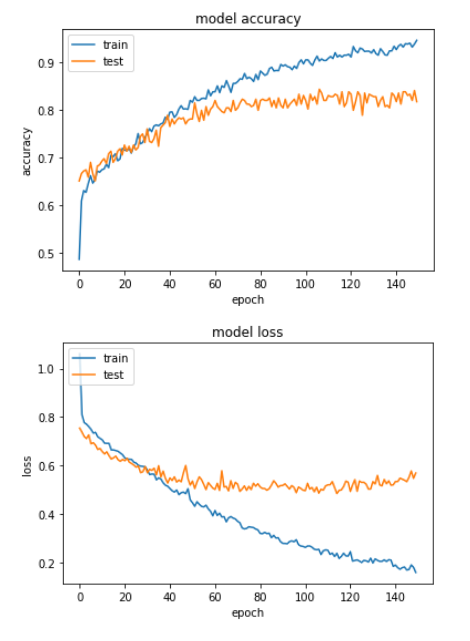
\includegraphics[width=\columnwidth]{images/cnn-multi.png}}
\caption{Training results when using multiple classes.}
\label{cnn-multi}
\end{center}
\end{figure}

\subsubsection{Alternative: Different Topology}

We experimented with a lot of different typologies. But in all cases we got worse results while training. One of the ideas was that our network should perform better when we gradually dense all our nodes to the final two nodes. The network itself is identical to the final model, however we replace the last step where we dense in to two nodes with a multiple dense layers (128, 64, 16 and 2). This gave us a better result on our training set but did not improve accuracy (fig. \ref{cnn-second}).

\begin{figure}[ht]
\begin{center}
\centerline{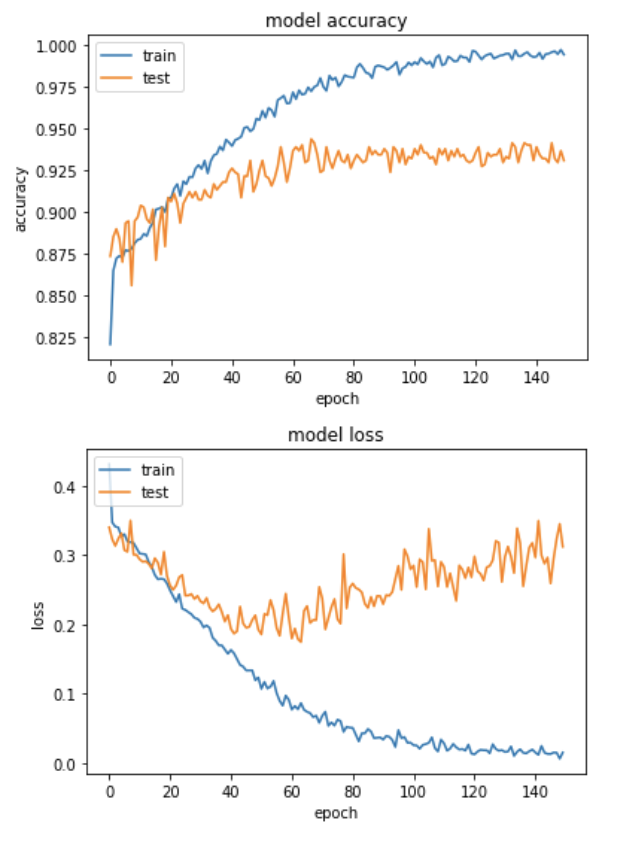
\includegraphics[width=\columnwidth]{images/cnn-training-second.png}}
\caption{Alternative approach to CNN using multiple dense layers.}
\label{cnn-second}
\end{center}
\end{figure}

Another attempt was to build a network using a small amount of filters compared to our original network, 6 and 16 compared to 32 and 64. The model quickly perfected the identification of training samples but performed awful on our test set (fig. \ref{cnn-naive}).

\begin{figure}[ht]
\begin{center}
\centerline{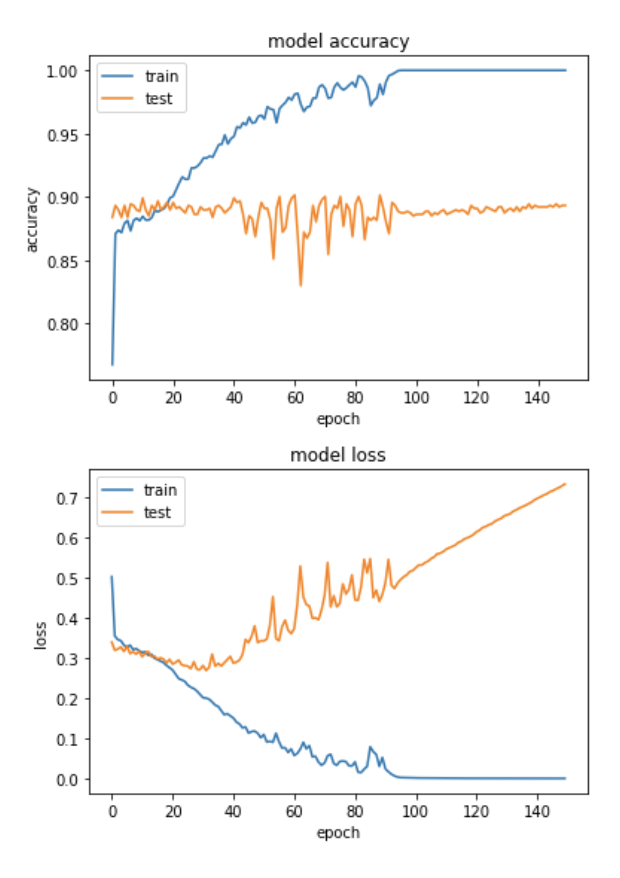
\includegraphics[width=\columnwidth]{images/cnn-training-naive.png}}
\caption{Alternative approach to CNN using less filters.}
\label{cnn-naive}
\end{center}
\end{figure}

\subsection{Detecting Ocean Tile}

Since land has buildings which show up as rectangular objects in our satellite imagery, this was labeled in most cases as being a ship/windmill. We had to remove land images from our data set to be able to train our model correctly.\\

Our first approach was to train a different neural network that would differentiate between land and ocean. This however seemed like a bigger task than we initially though and gave up on the idea after not achieving any good results. We tried to follow a method described by the University of Chinese Academy of Sciences (\cite{rs10122053}) but quickly realized this was beyond the scope of this project.\\

We started looking at different tools we could use to accurately define areas that are oceans. We found a project provided by Copernicus that has generated a land coverage map of every area on earth (\cite{copernicus}). By downloading a segment a using the imagery as a bitmap for masking oceans we can quickly exclude any tile that can't be a windmill. We added some padding to the edges land bodies to make sure beach features get excluded but this is not a reliable way of excluding beaches as beaches can vary on time related factors like tides.

\subsection{Clustering of ocean instances}

\subsubsection{Comparing clustering algorithms}

As we expect to see multiple windmills per park we can exclude the outliers. Boats or even anomalies detected in the ocean can be removed by using the proper clustering technique. Ordering points to identify the clustering structure (OPTICS) and density-based spatial clustering of applications with noise (DBSCAN) are algorithms for finding density-based clusters in spatial data. We assume the number of clusters relatively low and the density of the clusters rather similar, therefore we tend to use the DBSCAN technique. However we tried the OPTICS clustering method as well with multiple values for the hyper-parameters. 

\begin{figure}[ht]
\begin{center}
\centerline{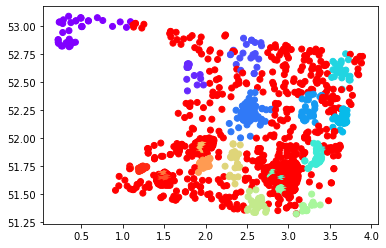
\includegraphics[width=\columnwidth]{images/cluster_optics.png}}
\caption{OPTICS Clustering result.}
\label{OPTICS Clustering}
\end{center}
\end{figure}

It is clear that the DBSCAN clustering technique produced a result much more in the line we'd expect. 

\begin{figure}[ht]
\begin{center}
\centerline{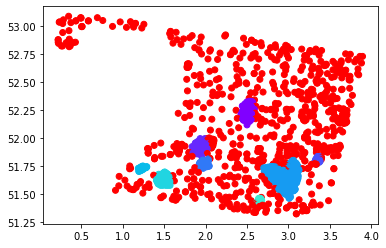
\includegraphics[width=\columnwidth]{images/cluster_dbscan.png}}
\caption{DBSCAN Clustering result.}
\label{DBSCAN Clustering}
\end{center}
\end{figure}

\subsubsection{Creating a boundary shape}

Create final shape as output of our pipeline

\subsection{Pipeline Overview}

Show a topology of our work. Link previous subsections together.

